%!TEX root = P231_notes.tex

\section{Dimensional Analysis}
\lecdate{lec~03}

You may be be surprised how far you can go in physics by thinking deeply about dimensional analysis. Here we’ll only get you started. To go one step further, you may read more about the Buckingham Pi theorem\footnote{\url{https://aapt.scitation.org/doi/10.1119/1.1987069}} or dive into neat applications\footnote{\url{https://aapt.scitation.org/doi/full/10.1119/1.3535586}, \url{http://inspirehep.net/record/153032?ln=en}}.
%

\subsection{Converting Units}

Imagine that you have three apples. This is a number (three) an a unit (apple). The meaning of the unit depends on what you’re using it to measure. For example, if apples are \$1 each, then you could use an apple as a unit of currency. The way to do this is to simply \emph{multiply by one}:
\begin{align}
  (3\text{ apples}) \times \left(\frac{\text{\$ 1}}{\text{apple}}\right)
  &= \$ 3 \ .
\end{align}
We have used the fact that the exchange rate is simply the statement that
\begin{align}
  1\text{ apple} &= \$1
  & \Rightarrow &&
  1 &= \frac{\$ 1}{1\text{ apple}} \ .
\end{align}
You can do a similar thing for [kilo-]calories or any other conversion rate. 


All that matters is that the conversion is constant. Indeed, the constants of nature make very good `exchange rates.' For example, in high-energy physics we like to use \textbf{natural units}. This is the curious statement that
\begin{align}
  \hbar = c = 1 \ .
\end{align}
At face value, this doesn’t make sense. $\hbar$ has units of action, $c$ is a speed, and 1 is dimensionless. However, because nature gives us a \emph{fundamental} unit of action and a \emph{fundamental} unit of speed, we may use them as conversion factors (exchange rates),
\begin{align}
  c = 3 \times 10^{10}~\text{cm}/\text{s} \ .
\end{align}
If $c=1$, then this means
\begin{align}
  1 \text{ s} &=  3 \times 10^{10}~\text{cm} \ .
\end{align}
This, in turn, connects a unit of time to a unit of distance. By measuring time, the constant $c$ automatically gives us an associated distance. The physical relevance of the distance is tied to the nature of the fundamental constant: one second (or `light-second') is the distance that a photon travels in one second. Observe that this only works because $c$ is a constant. 

\subsection{Quantifying units}

We use the notation that a physical quantity $Q$ has \textbf{dimension} $[Q]$ that can be expressed in terms of units of length, mass, and time:
\begin{align}
  [Q] = L^a M^b T^c \ .
\end{align}
The {dimension} is the statement of the powers $a$, $b$, and $c$. You may want to also include units of, say, electric charge. Sticklers may pontificate about whether electric charge formally carries a new unit or not. 

\begin{example}
What are the units of force? We remember that $\vec{F} = m\vec{a}$, so 
\begin{align}
  [\vec F] &= [m][\vec{a}] = M\times L T^{-2} = L^1 M^1 T^{-2} \ .
  \label{eq:02:force:units}
\end{align}
\end{example}

Life is even easier in \textbf{natural units}, where $c=1$ means that units of length and time are `the same’ and $\hbar = 1$ means that units of time and energy (mass) are inversely related. In natural units, one typically write $[Q]$ to mean the mass-dimension of a quantity. To revert back to conventional units, one simply multiplies by appropriate factors of $1=c$ and $1=\hbar$. 

\begin{example}
What are the units of force in natural units? From \eqref{eq:02:force:units} we multiply by one to convert length and time into mass dimensions:
\begin{align}
  [\vec F] &= [c^{-3} \hbar \vec{F}] = M^2 \ .
\end{align}
In natural units we say $[\vec F] = 2$. Recall that energy and mass have the same dimension, which you may recall from the Einstein relation $E^2 = m^2c^4 + p^2c^2$.
\end{example}


\subsection{Usage: Sanity Check}

The simplest use of dimensional analysis is to check your work. The following expression is obviously wrong:
\begin{align}
  1 + (3~\text{cm}) \ .
\end{align}
This does not make sense. You cannot sum terms with different dimensions. Similarly, $\sin(3\text{ cm})$ does not make sense. What about $e^{5~\text{cm}}$? This doesn't make sense because
\begin{align}
  e^x = 1 + x + \frac{1}{2!} x^2 +  \cdots
\end{align}
Since each term comes with a different power of $x$, the argument of the exponential must be dimensionless. 

\begin{exercise}
Consider the energy spectrum of light emitted from some constant source---a distant star, the ongoing annihilation of dark matter in the galactic center, a laser in the Hemmerling lab. The spectrum encodes how many photons are emitted per unit time. We can plot this spectrum as a curve on a graph. We can even normalize the curve so that it integrates to one photon. This means we only care about the distribution of energy, not the absolute amount. The horizontal axis of such a plot is the photon energy. What are the units of the vertical axis?
\end{exercise}


\subsection{Usage: Solving problems}

Here’s a common problem in introductory physics. Assume you have a pendulum with some [sufficiently small] initial displacement $\theta_0$. What’s the period, $\tau$ of the pendulum? We draw a picture like this:

\begin{center}
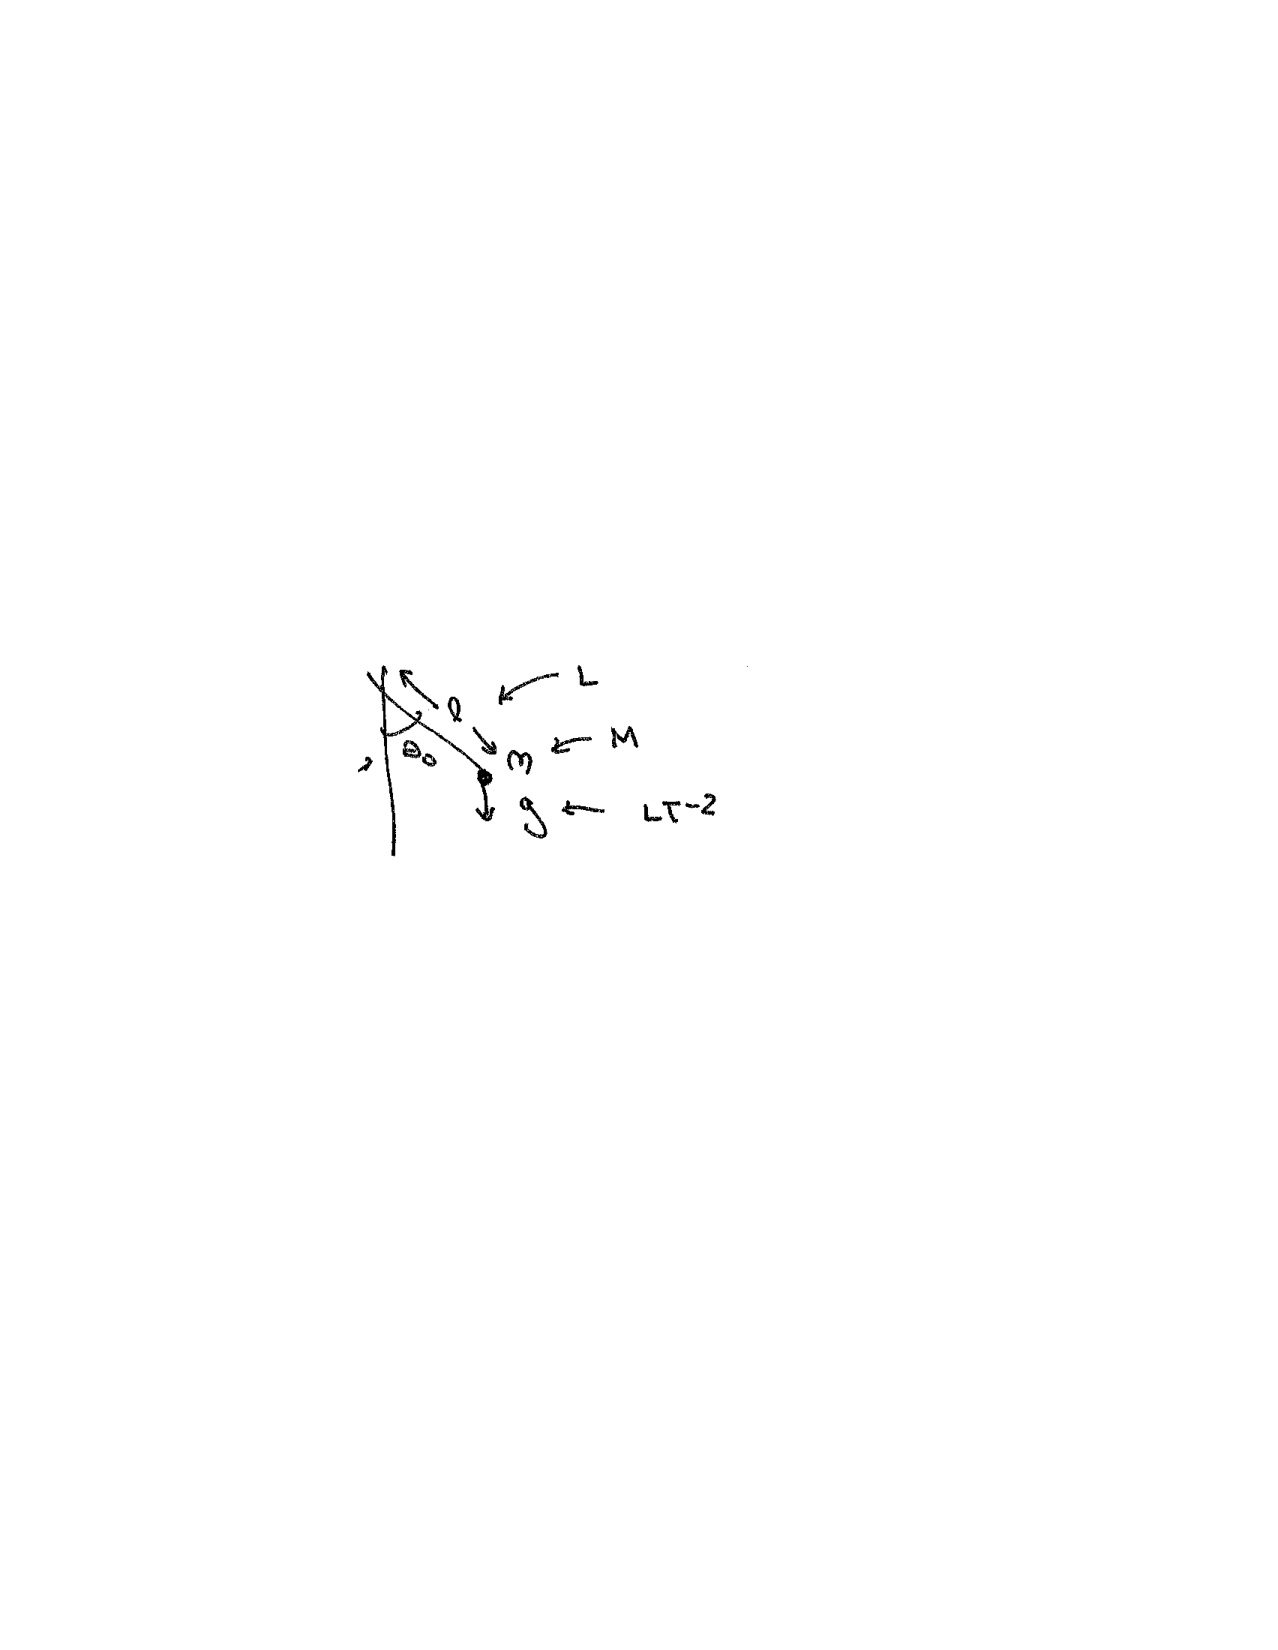
\includegraphics[width=.4\textwidth]{figures/lec01_pendulum.pdf}
\end{center}
%
From dimensional analysis, we know that the period has dimensions of time, $[\tau] = T$. The problem gives us a length $[\ell]=L$ and the gravitational acceleration, $[g]=LT^{-2}$. Note that $[\theta_0] = 1$ is dimensionless. This means that the only way to form a quantity with dimensions of time is to use $g^{-1/2}$. This leaves us with a leftover $L^{-1/2}$, which we can fix by inserting a square root of $\ell$:
\begin{align}
  \tau \sim g^{-1/2} \ell^{1/2} \ .
\end{align}
If we wanted to be fancy, we can make this an equal sign by writing a function of the other dimensionless quantities in the problem:
\begin{align}
  \tau = f(\theta_0) \sqrt{\frac{\ell}{g}} \ .
\end{align}


\subsection{Scaling}

A large part of physics has to do with scaling relations. Here’s a somewhat contrived example of how this works\footnote{This is adapted from section 11 of V.\ I.\ Arnold's \emph{Mathematical Methods of Classical Mechanics}, one of my favorite differential geometry textbooks because it's disguised as a book on mechanics.}. Suppose you have some static, central potential $U(\vec r)$. Maybe it’s some planet orbiting a star. 

\begin{center}
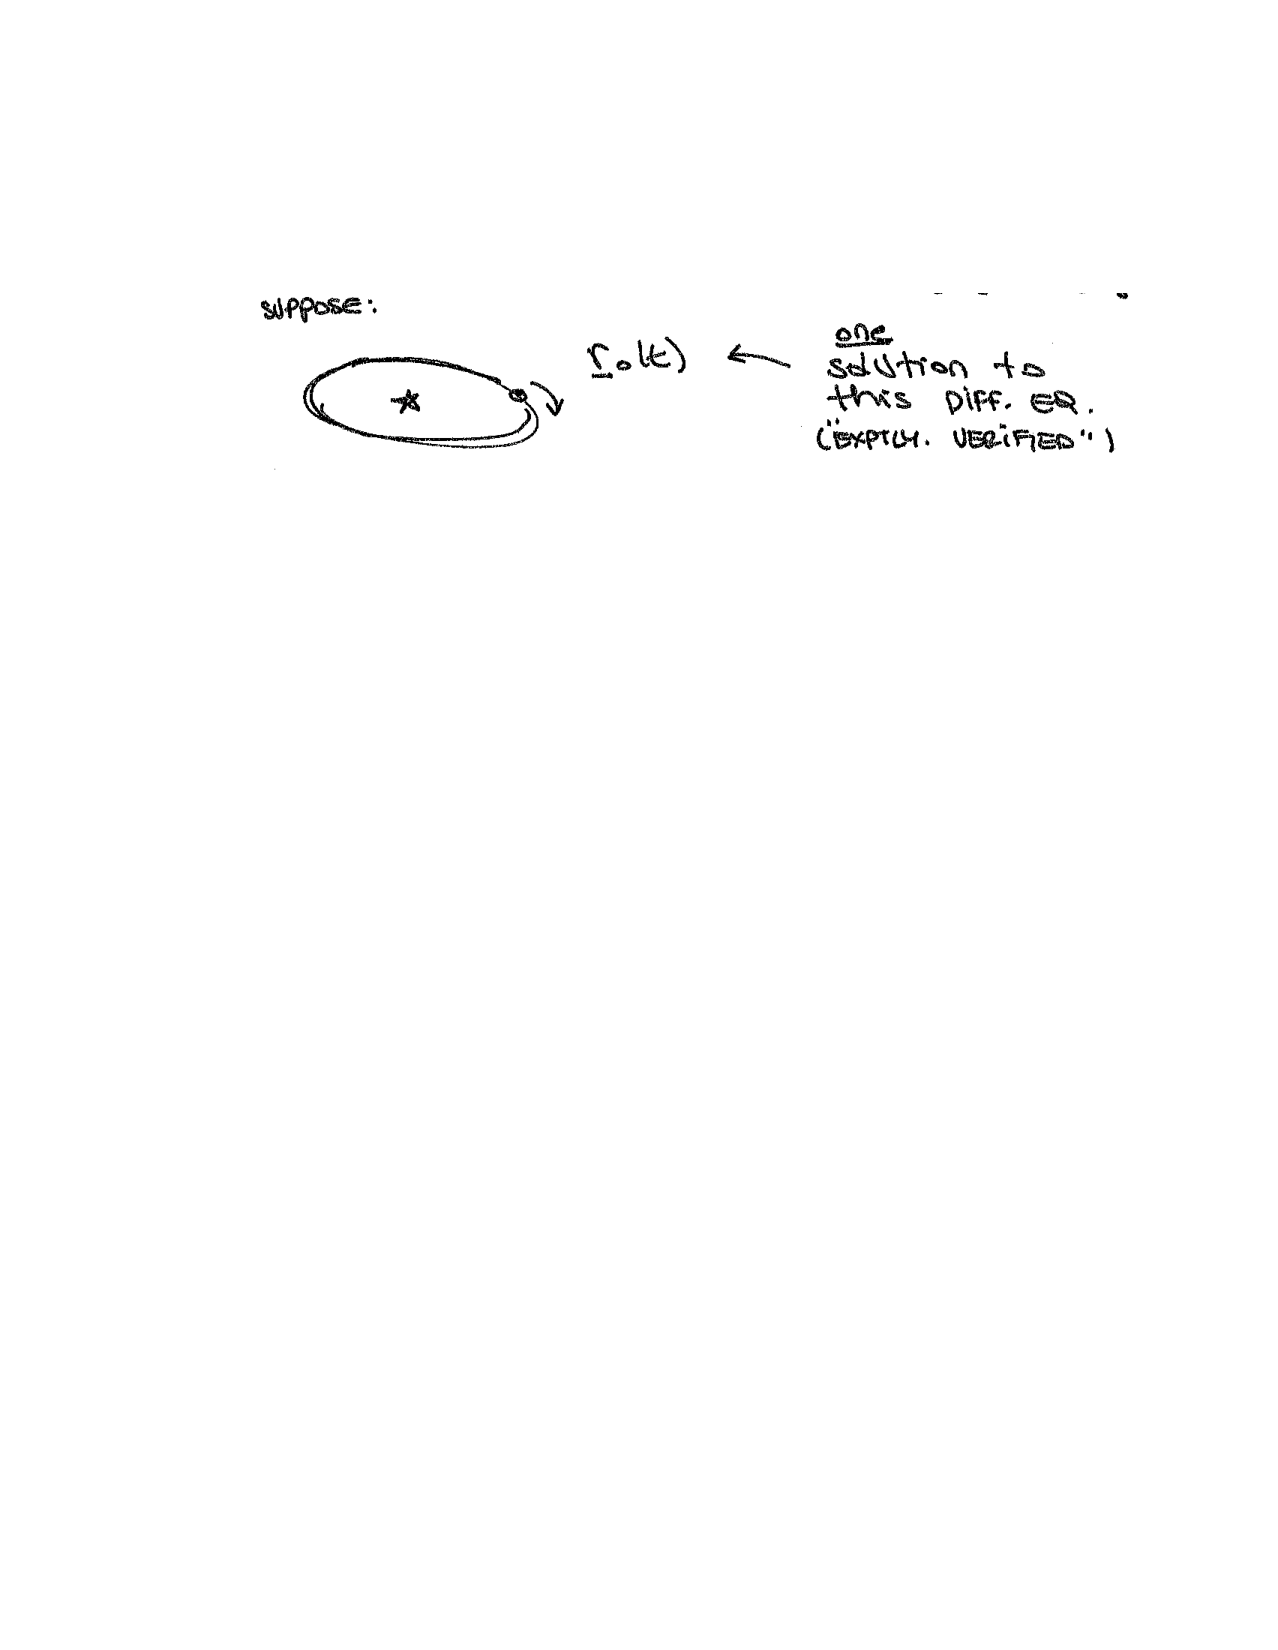
\includegraphics[width=.7\textwidth]{figures/lec01_orbit.pdf}
\end{center}

The force law gives:
\begin{align}
  m 
  \ddot{\vec{r}} = - \frac{\partial U}{\partial\vec{r}} \ .
  \label{eq:scaling:eg}
\end{align}
Suppose we are given a solution, $\vec r_0(t)$. Perhaps this is a trajectory that is experimentally verified. Dimensional analysis gives a way to scale this solution into other solutions. For example, let us scale time by defining a new variable $t'$:
\begin{align}
  t \equiv \alpha t' \ .
\end{align}
If the potential is static, then only the left-hand side of the force law changes. Even though the right-hand side formally has dimensions of time $\sim T^{-2}$, it does not transform because those units are carried in a constant, perhaps $G_N$, not a $(d/dt)^2$ like the left-hand side. The left-hand side of the force law gives:
\begin{align}
  m\left(\frac{d}{dt}\right)^2 \vec r_0(t) 
  &=
  m\alpha^{-2} \left(\frac{d}{dt'}\right)^2 \vec r_0(\alpha t') \ .
\end{align}
This begs us to define a new mass $m' = m\alpha^{-2}$. We thus have
\begin{align}
   m' \left(\frac{d}{dt'}\right)^2 {\vec{r}_0}(\alpha t')
  = - \frac{\partial U}{\partial\vec{r}_0} \ .
\end{align}
What this tells us is that $\vec r_1(t') \equiv \vec{r}_0(\alpha t')$ is a solution in the same potential that traces the same trajectory but at $\alpha$ times the speed and with mass $m'$. Changing labels $t'\to t$ for a direct comparison:
\begin{align}
   m' \left(\frac{d}{dt}\right)^2 {\vec{r}_1}(t)
  = - \frac{\partial U}{\partial\vec{r}_1} \ ,
\end{align}
which is indeed\footnote{We were able to swap $\vec r_0$ with $\vec r_1$ simply because $U$ only depends on the position.} \eqref{eq:scaling:eg} with a new mass $m'$ and a trajectory $\vec r_1(t') \equiv \vec{r}_0(\alpha t')$. For example, if $\alpha = 2$, then $\vec r_1(t)$ traces the same trajectory at double the velocity with one fourth of the mass. 

\subsection{Error Estimates}

This section is based on a lovely \emph{American Journal of Physics} article by Craig Bohren.\footnote{\url{https://doi.org/10.1119/1.1574042}} Let’s go back to another high school physics problem. 

\begin{center}
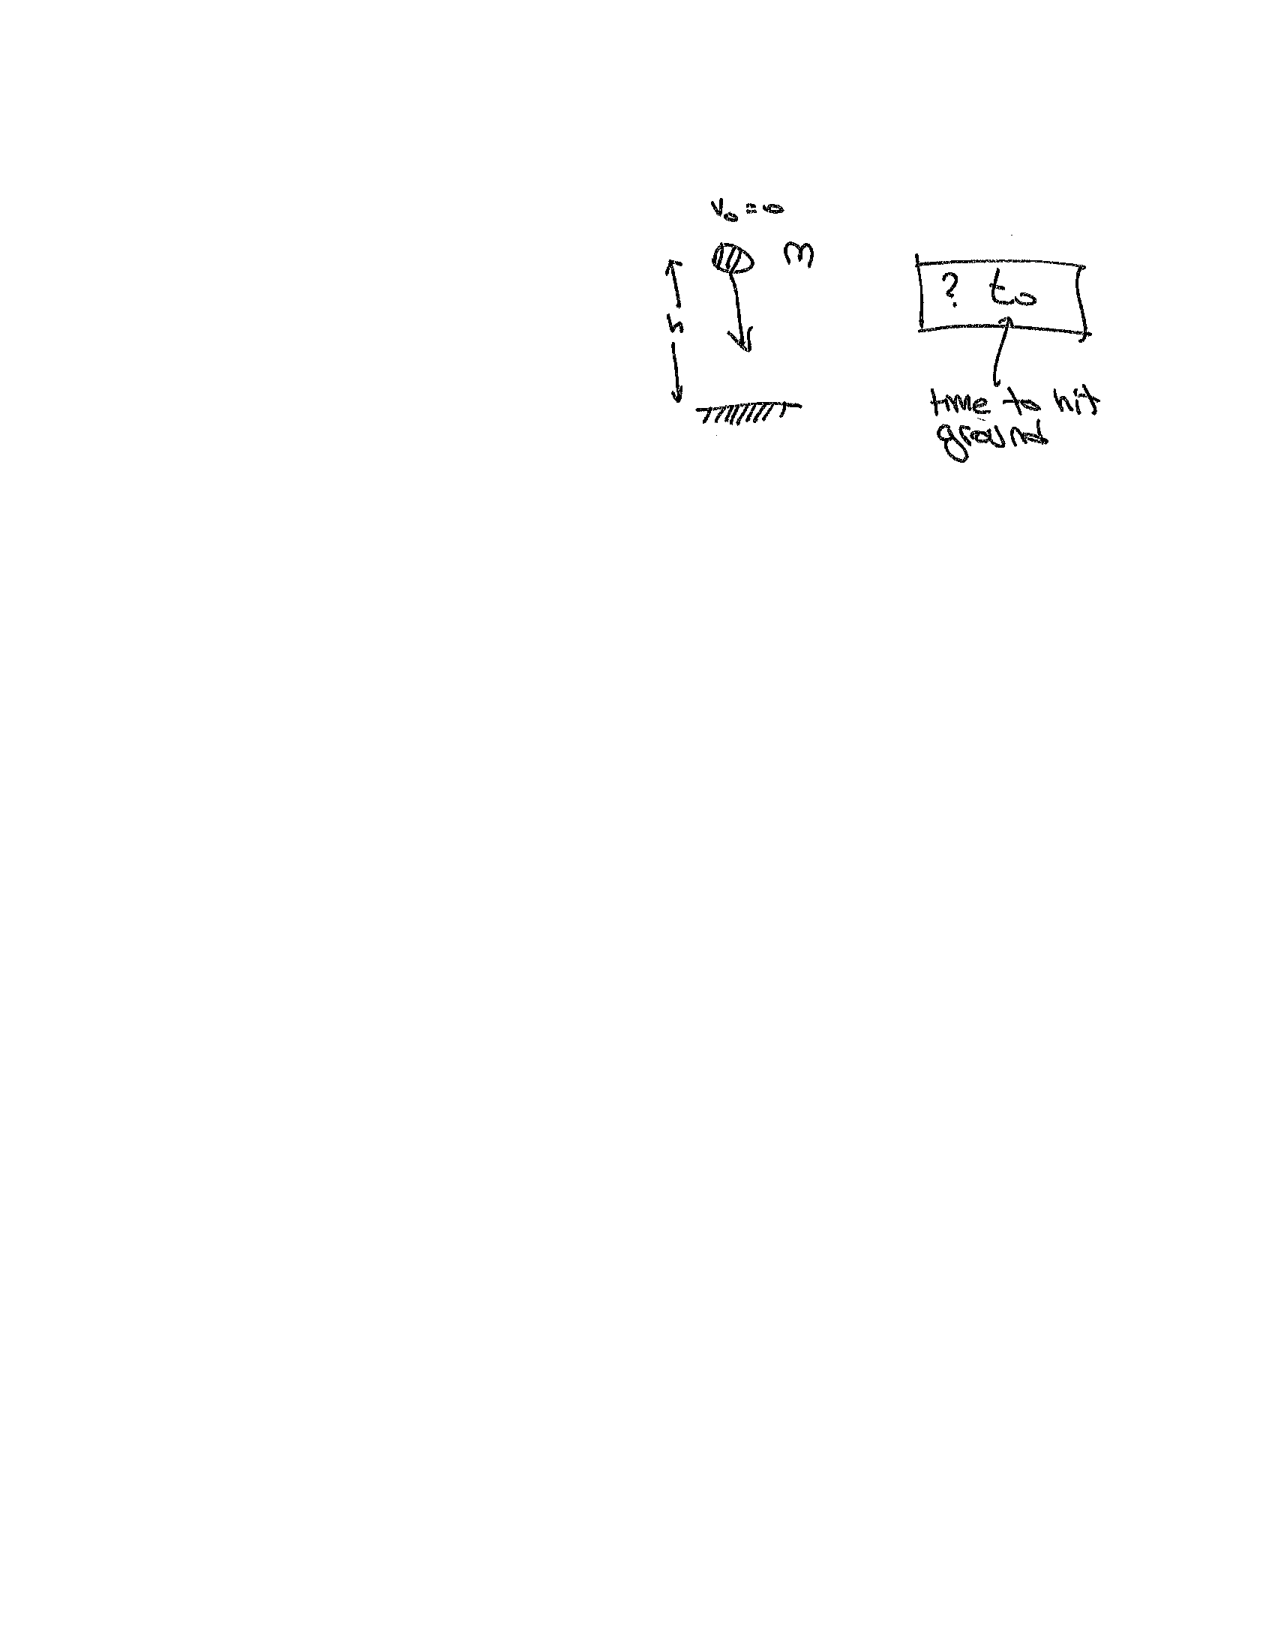
\includegraphics[width=.4\textwidth]{figures/lec01_drop.pdf}
\end{center}

Suppose you drop a mass $m$ from height $h$ that is initially at rest. How long before this hits the ground? You can integrate the force equation to get
\begin{align}
  t_0 = \sqrt{\frac{2h}{g}} \ .
\end{align}
This is the \emph{exact} answer \emph{within our model} of the system. The model made several assumptions. The mass is a point mass, the gravitational acceleration is constant at all positions, there is no air resistance, etc. In fact, we \emph{know} that if we do an experiment, our result will almost certainly \emph{not} be $t_0$. All we know is that $t_0$ is probably a good approximation of what the actual answer is.

\emph{How good of an approximation is it?}

One way to do this is to do the next-to-leading order (`NLO‘) calculation, taking into account a more realistic (and hence more complicated) model and then compare to $t_0$. But this is stupid. Why do we need to do a \emph{hard} calculation to justify doing an \emph{easy} one? If we’re going to do the hard calculation anyway, what’s the point of ever doing the easy one?

What we really want is an error estimate. The error is
\begin{align}
  \epsilon &= \frac{t_1 - t_0}{t_0} \ .
\end{align}
This is a dimensionless quantity that determines how far off $t_0$ is from a more realistic calculation, $t_1$. Ideally we don’t actually have to do work to get $t_1$. 

Let’s assume that we’re not completely nuts and that we’re in a regime where the error is small\footnote{Note the error has to be dimensionless in order for us to be able to call it `small,` otherwise it begs the question of `small with respect to what?`}. Then the error is a function of some dimensionless parameters, $\xi$, in the system. We define these $\xi$ so that as $\xi \to 0$, $\epsilon(\xi) \to 0$. In other words, the approximation gets better as the $\xi$ are made smaller. By Taylor expansion:
\begin{align}
  \epsilon(\xi) = \epsilon(0) + \epsilon'(0) \xi + \mathcal O(\xi^2) \ .
\end{align}
By assumption  $\epsilon(0) = 0$ and $\mathcal O(\xi^2)$ is  small. We can then make a reasonable \emph{assumption} that the dimensionless value $\epsilon'(0)$  is $\mathcal O(1)$. This tells us that the error goes like $\epsilon(\xi) \sim \xi$.

By the way $\mathcal O(1)$ is read ``order one'' and is fancy notation for the order of magnitude. Numbers like 0.6, 2, and $\pi$ are all $\mathcal O(1)$. A number like $4\pi^2$, on the other hand, is $\mathcal O(10)$.  The assumption that a dimensionless number is $\mathcal O(1)$ is reasonable. When nature gives you a dimensionless parameter that is both (a) important and (b) very different from $\mathcal O(1)$, then there's a good chance that it's trying to tell you something about your model. Good examples of this are the cosmological constant, the strong \acro{CP} phase, and the electroweak hierarchy problem\footnote{There are also `bad' examples. The ratio of the angular size of the moon to the angular size of the sun is unity to very good approximation. This is quite certainly a coincidence. Our universe appears to be in an epoch where the density of matter, radiation, and dark energy all happen to be in the same ballpark. Our cosmological models imply that this is purely a coincidence. It would be very curious if this were not the case. As an exercise, you can explore (and critique) the appearance of the anthropic principle in physics.}. 

Here’s how it works in practice. One effect that we miss in our toy calculation of $t_0$ is that the earth is round with radius $R$. This means that assuming a constant $g$ is an approximation. We have two choices for a dimensionless parameter $\xi$:
\begin{align}
  \xi &= \frac{h}{R}
  &\text{or}&&
  \xi &= \frac{R}{h} \ .
\end{align}
There is an obvious choice: $\xi = h/R$, because we know that as $h$ is made smaller (drop the ball closer to the ground) or $R$ becomes bigger (larger radius of Earth) then the constant $g$ approximation gets better. We thus expect that the corrections from the position-dependence of $g$ go like $\mathcal O(h/R)$.
 
% Exercise: check by explicit calculation, 2017 lec 1


\subsection{Bonus: Allometry}

There’s a fun topic called \textbf{allometry}. This is basically dimensional analysis applied to biology. A typical example is to consider two people who have roughly the same shape but different characteristic lengths, $\ell$ and $L$:

\begin{center}
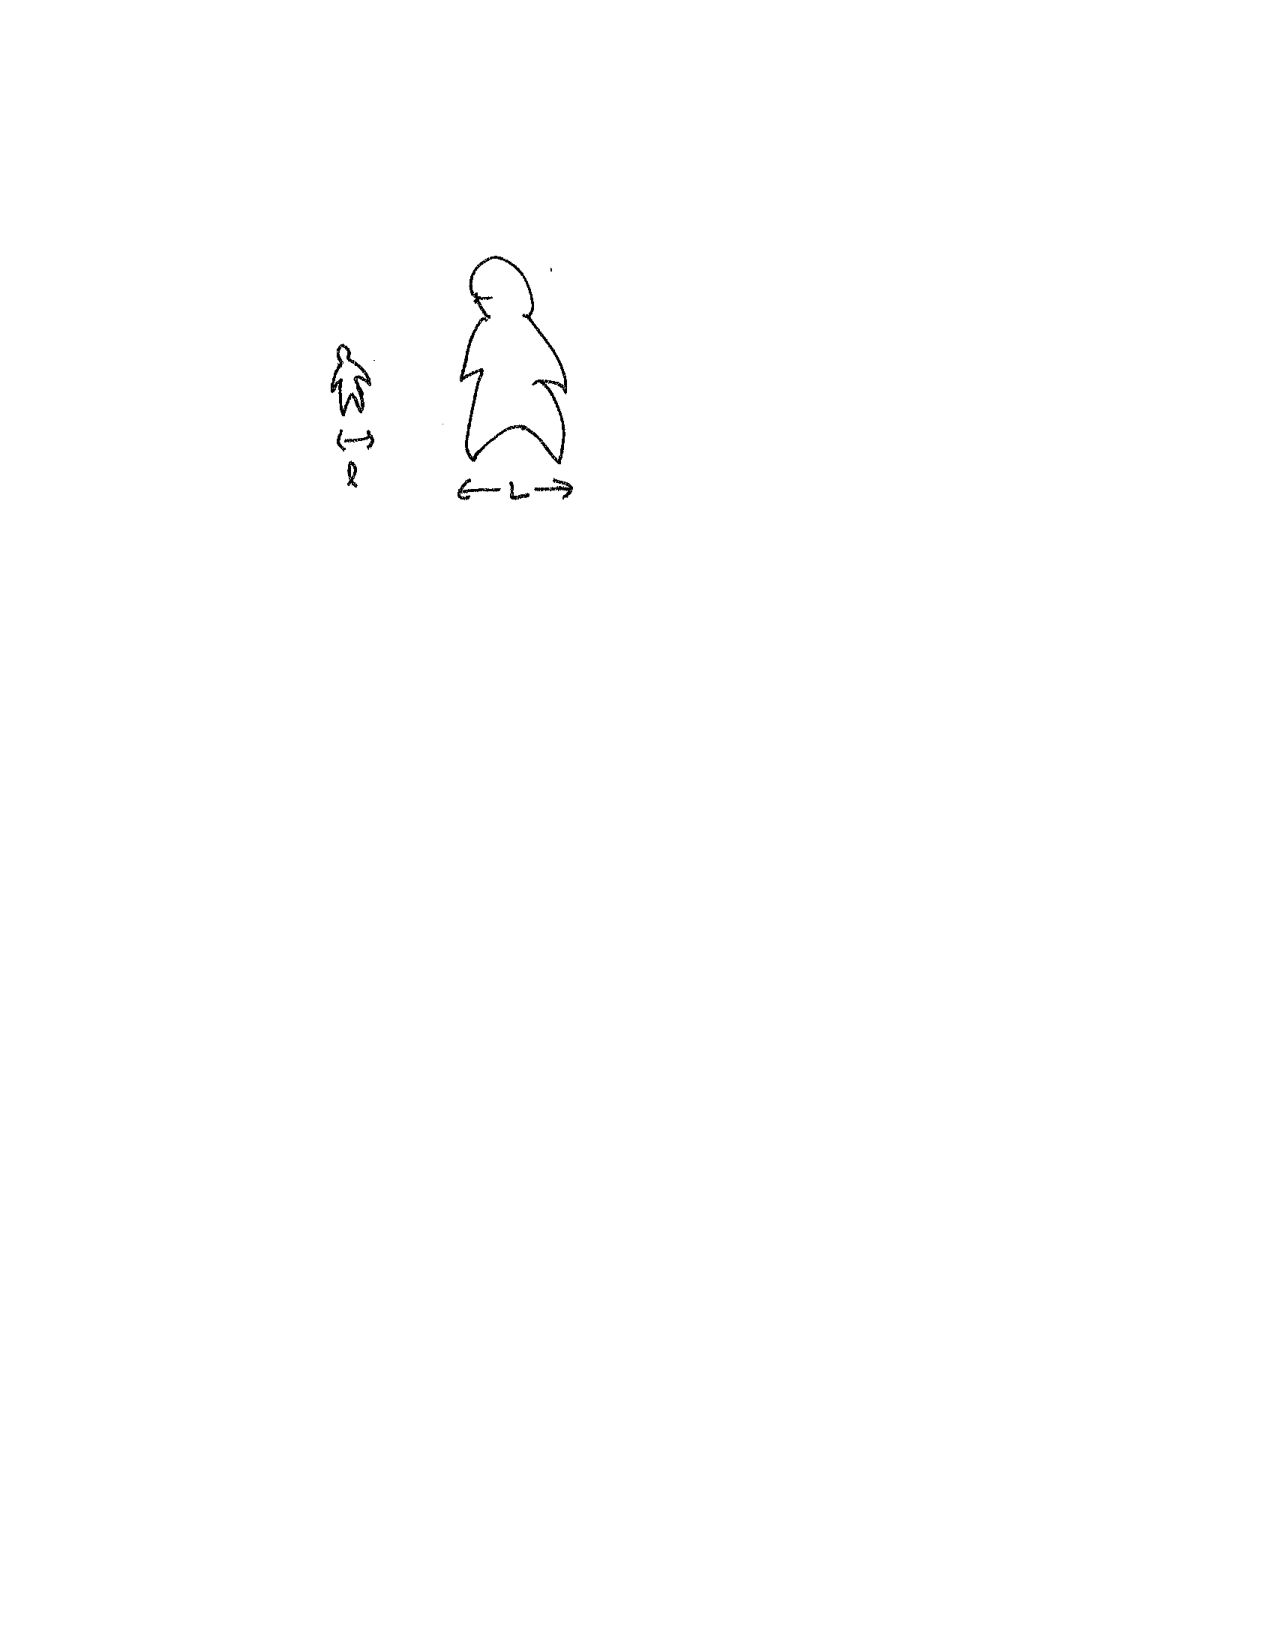
\includegraphics[width=.4\textwidth]{figures/lec01_allometry.pdf}
\end{center}

\begin{exercise}
If both people exercised at the same rate, which one loses more absolute weight? By how much? Let’s assume that weight loss is primarily from the conversion of organic molecules into carbon dioxide. 
\end{exercise}


\begin{exercise}
David Hu won his first IgNobel prize for determining that mammals take about 21 seconds to urinate, largely independently of their size\footnote{I learned about this in his excellent popular science book, \emph{How To Walk on Water and Climb Up Walls}.}. Can you use dimensional analysis to argue why this would be the case? It may be helpful to refer to the paper\footnote{\url{https://doi.org/10.1073/pnas.1402289111}}; as you read this, figure out which terms are negligible (and in what limits), identify the assumptions of the mathematical model (scaling of the bladder and urethra), and prove the approximate scaling relation. Make a note to yourself of which steps were non-trivial and where one may have naively mis-modeled the system. By the way, David Hu won a second IgNobel prize for understanding how wombats poop.
\end{exercise}